\documentclass{amsart}

%     If your article includes graphics, uncomment this command.
\usepackage{graphicx}
\usepackage{amsmath,amsfonts,amssymb,amscd,amsthm,amsbsy,upref}
\usepackage[all]{xy}
\usepackage{amsmath}
\usepackage{mathrsfs}
\usepackage{paralist}
\usepackage{setspace}
\usepackage{graphicx}
\usepackage{tikz-cd}
\usepackage{pgfplots}
\usepackage{fancyhdr}
\usepackage{tikz}
\usepackage{pgfplots}
\usepackage{array}

\newtheorem{theorem}{Theorem}[section]
\newtheorem{lemma}[theorem]{Lemma}

\theoremstyle{definition}
\newtheorem{definition}[theorem]{Definition}
\newtheorem{example}[theorem]{Example}
\newtheorem{xca}[theorem]{Exercise}

\theoremstyle{remark}
\newtheorem{remark}[theorem]{Remark}

\numberwithin{equation}{section}

%    Absolute value notation
\newcommand{\abs}[1]{\lvert#1\rvert}

%    Blank box placeholder for figures (to avoid requiring any
%    particular graphics capabilities for printing this document).
\newcommand{\blankbox}[2]{%
  \parbox{\columnwidth}{\centering
%    Set fboxsep to 0 so that the actual size of the box will match the
%    given measurements more closely.
    \setlength{\fboxsep}{0pt}%
    \fbox{\raisebox{0pt}[#2]{\hspace{#1}}}%
  }%
}

\pgfplotsset{compat=1.13}

\begin{document}

\title{Assigning Scouts to Optimal Patrols}
\author{Phil Snyder}
\author{Ian Bruce}
\author{Julio Marco Pineda}

\begin{abstract}
The Scoutmaster wants to find an arrangement of 13 new scouts into two patrols. The cohesiveness and overall quality experience of a patrol is severely affected by adverse relationship and can be improved by existing preferences. Thus, by using anonymous data from scouts and parents, a brute force strategy was employed to find the optimal arrangement of scouts that avoids severe conflict and maximizes existing preferences. An arrangement of 6 and 7 scouts on one patrol respectively was found that satisfies the desired conditions. 
\end{abstract}
\maketitle
\section*{Problem Description}
Every year the Scoutmaster must assign new scouts to groups called patrols. In these patrols, scouts would plan and perform different scouting activities together in which they can form close friends that grow together. However, in recent years, the number of scouts have been increasing at a rate such that it is no longer logistically viable to place every new scout in a single patrol; multiple patrols are needed to organize activities better and to form proper bonds and community between the new recruits. Furthermore, the new scouts are in the fifth or sixth grade who have not fully developed their interpersonal skills. Many can be temperamental and awkward when dealing with adversity, and even some devastating conflicts occur where not only the two fighting scouts create animosity between each other, the rest of the troop alienates the destructive pair. If enough of these adverse interactions occur within a troop, many scouts would decide to quit and lose out in a great experience and community in the Boy Scouts.

The data the scoutmaster collects about adverse pairings and preferences are either privately given by the scouts themselves or by their parents. The possibly destructive interactions are given by the parents of the scouts.Previously, the Scoutmaster was able to determine the perfect patrols manually due to having smaller number of scouts. However, the number of scouts have been increasing yearly to the point that solving this grouping problem cannot be done by hand in a reasonable time. Therefore, we can help our community partner find a better means to solve his troop organization problem. Our goal for this project is to assign boy scouts in different patrols of appropriate size (of 6-8 scouts) such that we maximize the retention rate of the scouts in the program by avoiding severe conflicts while maximizing positive relationships between scouts.

We would like to answer the direct problem our community partner provided of arranging 15 scouts into two troops that avoids severe conflicts and promotes the positive relationships between the scouts. Furthermore, we want to determine if we can build a model to predict these patrol arrangements for any number of scouts so that the Scoutmaster can use this model for future years. Other than improving the overall experience of the scouts and alleviating the burden of the Scoutmaster, this model can possibly be applied to other situations where arranging a number of people of groups where interpersonal dynamics is necessary and important.

\section*{Simplifications}
Ultimately, our goal is to find groups for the scouts that will allow them to grow and be happy in the troop. If we really wanted to fully understand how a group can foster growth in an individual, we would want to consider the astronomical number of aspects about the personalities of each member and how those influence each of the other members given those other members’ astronomically complex personalities. Sociological and psychological literature would need to be studied extensively to learn about these aspects, and experts in the field would most likely be required to collect relevant data for each child, taking several weeks to conduct interviews. At the of the day, given our limited knowledge in this area, we settled with considering a subset of the sociological data between the scouts. We asked each scout which other scouts they liked and which ones they disliked. Now, this is obviously a giant simplification, but the difficulty of gathering more complex information and compiling said information would be too great for the expertise level of anyone involved in solving this problem. Also, this process of gathering data would have to be repeated each year for each new batch of new scouts, and would therefore be a burden on the Scoutmaster to collect a lot of data.

Another simplification is to assume that the quality of a group can be determined by the quality of the relationships between the unique pairs of the group - in other words, the whole is equal to the sum of the parts. For example, consider the case where scouts A, B and C individually like each other when they are alone with one other scout, but don’t like being in a group together. This epiphenomenon won’t be considered; in context of our model, the pairing of these scouts would be heavily favored. 

\section*{Mathematical Model}
To model the relationships between scouts, we use a mathematical graph. We let the scouts be vertices in our graph. A directed edge between Scout A and Scout B has a weight proportional to how much Scout A likes Scout B. We would then like to find a partition of the vertices in the graph that minimizes an objective function given constraints on the sizes of subsets generated by our partition. This results in a complete graph on 13 vertices having edge weights 0, 1, or -1, corresponding to indifference, approval, or disapproval, respectively. Scoutmaster Bruce specifically would like two patrols from the 13 scouts - one of size 6, the other of size 7. The total number of partitions given these constrants is $\binom{13}{6} = \binom{13}{7} = 1716$. This number is reasonable enough that we may calculate the total loss of every valid grouping and select the partition with the lowest score.

We measure the goodness (or score) of a partition in six different ways, corresponding to six different objective functions, which we dub MinCut, FriendCut, EnemyCut, AwkwardCut, and HybridCut. MinCut is designed to minimize the cut edge weights between partitions (see \textit{Solution of Mathematical Problem}). FriendCut is designed to maximize the number of intra-patrol positive edge weights. EnemyCut is meant to minimize the number of intra-patrol negative edge weights, Awkward cut ($+i$) is the same as MinCut, but with an additional penalty of $i$ if there are a pair of scouts, Scout A and Scout B, such that Scout A favors Scout B, but Scout B disfavors Scout A. Hybrid Cut is a convex combination of MinCut and FriendCut, each with equal weight (that is, half the MinCut loss plus half the FriendCut loss). Our three primary objective functions - MinCut, FriendCut, and EnemyCut are given a more rigorous treatment in the next section.

\section*{Solution of Mathematical Problem}
We represent our directed graph as a 13 by 13 similarity matrix, or, as might
be more fitting for the problem, an ``affinity'' matrix. Like below\footnote{The scouts were enumerated like so: 1. Brandon, 2. Cameron, 3, Christian, 4. Colby, 5. Daniel, 6. Darwin, 7. Evan, 8. Jake, 9. Jordan, 10. Nathan, 11. Patrick, 12. Timmy, 13. Tommy.}:

\begin{figure}[h]
    \centering
    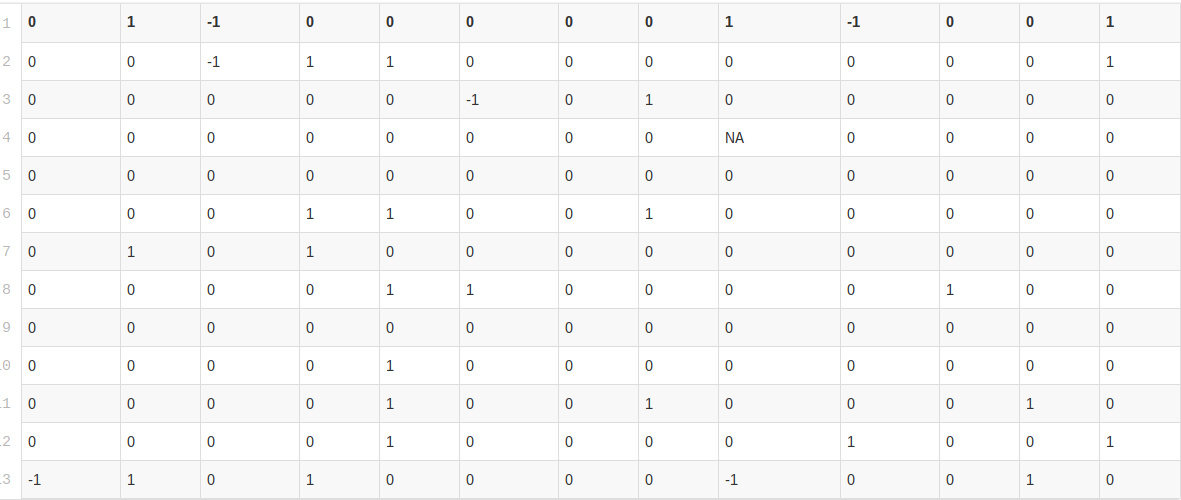
\includegraphics[scale=0.28]{data}
\end{figure}
%%%%%%%%%%%%%%%%%%%%%%%%%%%%%%%%%%%%%%%%%%%%%%%%%%%%%%%%%%%%%%%%%%%%%%%%
%%%%%%%%%%%%%%%%%%%%%%%%%%%%%%%%%%%%%%%%%%%%%%%%%%%%%%%%%%%%%%%%%%%%%%%%

The NA value represents a hard constraint established by a scout's parent (i.e., under no circumstances are these two to be in the same patrol). We designed a number of objective functions that accept two scouts and calculates the loss associated with such a placement. The loss is defined to be $L(x, y) = \text{max}(-2, x[y] + y[x])$ where $x[y]$ is $x$'s disposition towards $y$ and vise versa. For example, if $x$ dislikes $y$ and $y$ dislikes $x$, the loss is -2. If $x$ likes $y$ but $y$ dislikes $x$ the loss is 0. If $x$ and $y$ both like each other, the loss is 2. In mixed cases where the first scout is indifferent to another, but the other likes or dislikes the first scout, the loss is +1 or -1 respectively. We are trying to minimize the loss, so in applying our loss function over the entire dataset, our algorithm is equally averse to same-patrol mutual enmity as it is to dividing mutual friendship, half as averse to the indifference of one scout and the stronger inclination of another, and indifferent to polar opposite affinities within the same patrol. There is a question as to whether this is an accurate reflection of how individual scouts would view their own ``loss'' of any of the possible scenarios. As it turns out, our algorithm arrives at a very reasonable solution regardless. 
\section*{Results}
As mentioned earlier, the number of scouts we must partition is small enough to find an optimal solution by brute force. Our algorithm finds a partition of scouts into patrols of sizes 6 and 7 which is optimal with respect to each objective.

\clearpage

\begin{figure}[h]
\centering
\begin{tabular}{ |l|l|l|l|l|l| }
\hline
\multicolumn{2}{|c|}{\textbf{MinCut}} & \multicolumn{2}{|c|}{\textbf{FriendCut}} & \multicolumn{2}{|c|}{\textbf{EnemyCut}}\\
\hline
Patrol 1 & Patrol 2 & Patrol 1 & Patrol 2 & Patrol 1 & Patrol 2\\
\hline
Brandon & Christian & Brandon & Daniel & Brandon & Christian\\
Cameron & Daniel & Cameron & Darwin & Cameron & Jake\\
Colby & Jake & Christian & Jake & Colby & Jordan\\
Darwin & Jordan & Colby & Jordan  & Daniel & Nathan\\
Evan & Nathan & Evan & Nathan & Darwin & Patrick\\
Tommy & Patrick & Tommy & Patrick & Evan & Timmy\\
& Timmy & & Timmy & Tommy & \\
\hline
\multicolumn{6}{|c|}{\hphantom{1}} \\
\hline
\multicolumn{2}{|c|}{\textbf{AwkwardCut (+1)}} & \multicolumn{2}{|c|}{\textbf{AwkwardCut (+2)}} & \multicolumn{2}{|c|}{\textbf{HybridCut}} \\
\hline
Patrol 1 & Patrol 2 & Patrol 1 & Patrol 2 & Patrol 1 & Patrol 2\\
\hline
Brandon & Christian & Brandon & Cameron & Brandon & Christian\\
Cameron & Daniel & Christian & Evan & Cameron & Daniel\\
Colby & Jake & Daniel & Evan & Colby & Darwin\\
Darwin & Jordan & Darwin & Nathan & Evan & Jake\\
Evan & Nathan & Jake & Timmy & Timmy & Jordan\\
Tommy & Patrick & Jordan & Tommy & Tommy & Nathan\\
\hphantom{1} & Timmy & Patrick & \hphantom{1} & \hphantom{1} & Patrick\\
\hline
\end{tabular}
\caption{The partitions arrived at by minimizing each objective function}
\end{figure}

For each method we define three scoring metrics:

\begin{enumerate}
\item \textbf{MinCut}. This is the traditional metric of a cut on a weighted graph and is the sum of the weights of the edges we would ``cut'' if we were to sever the edges between distinct patrols. More formally, for some partition $I, J$ $I \neq J$, the MinCut is defined as:
$$
MinCut(I, J) := \sum_{e = (i, j), i \in I, j \in J}^{} c(e)
$$
We want this to be as low as possible.
\item \textbf{FriendCut}. This is the sum of the positive, or friendly edge weights within each patrol. That is, if $I_+ = \{e=(i,j) | i,j \in I, c(e)=1\}$ is the the set of edges in patrol $I$ with positive weight and $J_+ = \{e=(i,j) | i,j \in J, c(e)=1\}$ is the set of edges in patrol $J$ with positive weight, then (assuming all positive weights are 1):
$$
FriendCut(I, J) :=  |I_+ \cup J_+|
$$
We want this to be as high as possible.
\item \textbf{EnemyCut}. This is similar to FriendCut, except we now measure the number of negative edges going from one scout to another within the same patrol. Let $I_- = \{e=(i,j) | i,j \in I, c(e)=-1\}$ be the the set of edges in patrol $I$ with negative weight and $J_- = \{e=(i,j) | i,j \in J, c(e)=-1\}$ be the set of edges in patrol $J$ with negative weight, then
$$
EnemyCut(I, J) := |I_- \cup J_-|
$$
    We want this to be as low as possible.
\end{enumerate}

The other methods are modifications of these three and are defined in Appendix A.

\clearpage 

\begin{figure}[h]
    \centering
    \begin{tabular}{ |l|l|l|l| }
        \hline
        \textbf{Method} & \textbf{MinCut} & \textbf{FriendCut} & \textbf{EnemyCut} \\
        \hline
        MinCut & 0 & 17 & 0 \\
        FriendCut & 1 & 18 & 1 \\
        EnemyCut & 2 & 15 & 0 \\
        AwkwardCut (+1) & 0 & 17 & 0 \\
        AwkwardCut (+2) & 1 & 18 & 2 \\
        HybridCut & 0 & 18 & 1 \\
        \hline
    \end{tabular}
    \caption{The scores according to the three primary metrics.}
\end{figure}

Of the objective functions we chose to use, it seems like MinCut and HybridCut are the best performing. FriendCut performs almost as well as HybridCut, except for one worse in the EnemyCut objective. EnemyCut does poorly since finding a partition with 0 intra-patrol negative weight edges is easy in this example, and so EnemyCut settles for the first suboptimal (in terms of the other objective functions) solution it finds. AwkwardCut (+1) arrived at the same partition as MinCut (not altogether surprising, but informative, since even with the additional +1 penalty for placing Brandon and Tommy in the same patrol it decided it would be best off to do so anyways). But changing the ``awkward'' penalty to +2, the same penalty as mutual dislike in EnemyCut, we get a completely different partition.

Let's take a more critical look at the optimal partition arrived at via MinCut:

\begin{table}[h]
	\caption{}\label{eqtable}
	\renewcommand\arraystretch{1.5}
	\noindent\[
	\begin{array}{|c|c|}
	\hline
	\textbf{Patrol 1}&\textbf{Patrol 2}\\
	\hline
	\text{Brandon, Cameron, Colby,}&\text{Christian, Daniel, Jake,}\\
	\text{Darwin, Evan, Tommy}&\text{Jordan, Nathan, Patrick, Timmy}\\
	\hline
	\end{array}
	\]
\end{table}
\begin{figure}[h]
    \centering
    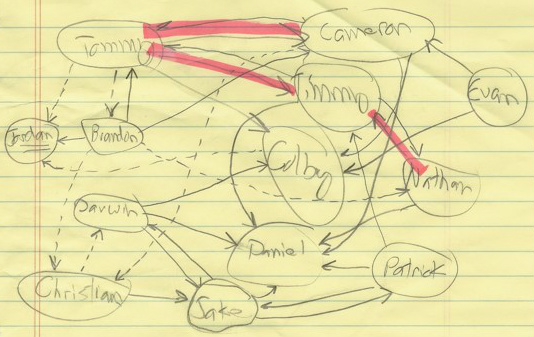
\includegraphics[scale=0.60]{graph}
\end{figure}

\begin{enumerate}
	\item Tommy and Timmy both like each other and are in separate patrols. But if we move Timmy to Patrol 1 ($P1$), we break up the mutual friendship of Timmy and Nathan in $P2$. Suppose we moved both Timmy and Nathan to $P1$ and Brandon (who dislikes Nathan) to $P2$. But then Brandon loses two friends (Tommy and Cameron), gains one (Jordan), and now neither Nathan nor Timmy are in the same patrol as Daniel, whom they both like. Although, Brandon and Tommy find themselves in the awkward situation of having complete opposite sentiments towards each other. Perhaps this would be a worthwhile trade after all (and a larger, negative weight needs to be placed upon disfavor-favor relationships).
	
	\item As mentioned in the previous point, Tommy dislikes Brandon. Trading Tommy in $P1$ for Jordan in $P2$ seems promising, But we have overlooked the fact that Colby and Jordan are our NA pair, and cannot be in the same patrol under any circumstances. Trading Colby for Jordan is another option, but Colby will be missed by Darwin, Evan, Cameron and Tommy (In other words, the whole of P1 minus Brandon).
\end{enumerate}

On the whole, though, there are no obvious improvements that can be made to our algorithm's partition. We find that this is an assignment that could have reasonably been arrived at by Scoutmaster Bruce (granted the group dynamics have not changed since the scouts were surveyed).  Furthermore, the solution took only 10 seconds to arrive at on a single core machine.

\section*{Improvements}
While our algorithm demonstrably works well on smaller groups of 13 people, we do not expect our brute force solution to be tractable on larger groups wherein greater than 2 partitions are required. As a possible scenario, consider a company of 150 people to be divided into fixed-size teams of 10 individuals each. There are $150! / (10!)^{15}$ possible partitions, a number proportional to $10^{164}$ - meaning we could instead use that computational time to enumerate the number of atoms in the universe… a tredecillion $(10^{78})$ times. Knowing this, perhaps it won’t surprise the reader that this particular graph partitioning problem in general graphs is NP-complete - though there do exist approximation algorithms.%
%%%%%%%%%%%%%%%%%%%%%%%%%%%%%%%%%%%%%%%%%%%%%%%%%%%%%%%%%%%%%%%%%%%%%%%%
\footnote{B. W. Kernighan, S. Lin, \textit{An Efficient Heuristic Procedure for Partitioning Graphs}. Bell System Technical Journal. \textbf{49} (1970), 291--307. doi: 10.1002/j.1538-7305.1970.tb01770.x}%
%%%%%%%%%%%%%%%%%%%%%%%%%%%%%%%%%%%%%%%%%%%%%%%%%%%%%%%%%%%%%%%%%%%%%%%%
As scout enrollment increases, it becomes necessary to consider scenarios where we have both a large number of scouts in need of assignment and multiple patrols to choose from. Our algorithm could be extended to use brute force to find a globally optimal solution when it is deemed computationally feasible and to use an approximating algorithm to find a locally optimal solution otherwise. 

\section*{Conclusions}
We initially struggled to decide on determining an appropriate objective function to partition the scouts to different groups. Follow up interviews with Scoutmaster Gene Bruce allowed us to decide on this function. We learned to rely on his expertise and intuition rather than trying to blindly decide on which types of relationships should be fostered and avoided to weight our objective function. Thus, we learned necessary communication skills and consideration of our community partner's needs.

With a feasibility check of how many solutions possible once the mathematical model was decided using graphs, a brute force strategy was the most accessible method to arrive at a solution. Thus we were able to develop a program that can partition scouts using this strategy. We learned to utilize tools we have at hand right away, and then we can consider other methods later on to reduce the computational time of our algorithm.

\section*{Acknowledgments}
We would like to thank Scoutmaster Gene Bruce for providing us the necessary data and being extremely patient and understanding when discussing the background and problem. We would also like to thank Professor Sarah Billey for the mentorship and guidance she provided throughout this project, and our TA Austin Tran for his comments and suggestions. 

\section*{Verification Statement}
(Once we receive our verification statement, we will place it here.)

\section*{Appendix A}
The other objective functions.

\begin{enumerate}
    \item \textbf{AwkwardCut (+i)}. Same in all respects to MinCut, except for an additional penalty of $i$ if there are two scouts, Scout A and Scout B, in the same patrol such that Scout A likes Scout B and Scout B dislikes Scout A.
    \begin{equation*}
        \begin{split}
            AwkwardCut&(I, J, i) := \Bigg[ \sum_{e = (k, j), k \in I, j \in J}^{} c(e) \Bigg] \\
            &+ i * \left\vert{\{e_+ = (k,j), e_- = (j, k) : e_+, e_- \in I, c(e_+) = 1, c(e_-) = -1\}}\right\vert
        \end{split}
    \end{equation*}

\item \textbf{HybridCut}. A convex combination of MinCut and FriendCut, each with equal weight (that is, half the MinCut loss plus half the FriendCut loss).
    \begin{equation*}
        HybridCut(I, J) := \frac{1}{2}MinCut(I, J) + \frac{1}{2}FriendCut(I, J)
    \end{equation*}
\end{enumerate}


\bibliographystyle{amsplain}
\begin{thebibliography}{10}

\bibitem {A} B. W. Kernighan, S. Lin, \textit{An Efficient Heuristic Procedure for Partitioning Graphs}. Bell System Technical Journal. \textbf{49} (1970), 291--307. doi: 10.1002/j.1538-7305.1970.tb01770.x

\end{thebibliography}

\end{document}

%------------------------------------------------------------------------------
% End of journal.tex
%------------------------------------------------------------------------------
=======

\documentclass{amsart}

%     If your article includes graphics, uncomment this command.
\usepackage{graphicx}
\usepackage{amsmath,amsfonts,amssymb,amscd,amsthm,amsbsy,upref}
\usepackage[all]{xy}
\usepackage{amsmath}
\usepackage{mathrsfs}
\usepackage{paralist}
\usepackage{setspace}
\usepackage{graphicx}
\usepackage{tikz-cd}
\usepackage{pgfplots}
\usepackage{fancyhdr}
\usepackage{tikz}
\usepackage{pgfplots}
\usepackage{array}

\newtheorem{theorem}{Theorem}[section]
\newtheorem{lemma}[theorem]{Lemma}

\theoremstyle{definition}
\newtheorem{definition}[theorem]{Definition}
\newtheorem{example}[theorem]{Example}
\newtheorem{xca}[theorem]{Exercise}

\theoremstyle{remark}
\newtheorem{remark}[theorem]{Remark}

\numberwithin{equation}{section}

%    Absolute value notation
\newcommand{\abs}[1]{\lvert#1\rvert}

%    Blank box placeholder for figures (to avoid requiring any
%    particular graphics capabilities for printing this document).
\newcommand{\blankbox}[2]{%
  \parbox{\columnwidth}{\centering
%    Set fboxsep to 0 so that the actual size of the box will match the
%    given measurements more closely.
    \setlength{\fboxsep}{0pt}%
    \fbox{\raisebox{0pt}[#2]{\hspace{#1}}}%
  }%
}

\pgfplotsset{compat=1.13}

\begin{document}

\title{Assigning Scouts to Optimal Patrols}
\author{Phil Snyder}
\author{Ian Bruce}
\author{Julio Marco Pineda}

\begin{abstract}
The Scoutmaster wants to find an arrangement of 13 new scouts into two patrols. The cohesiveness and overall quality experience of a patrol is severely affected by adverse relationship and can be improved by existing preferences. Thus, by using anonymous data from scouts and parents, a brute force strategy was employed to find the optimal arrangement of scouts that avoids severe conflict and maximizes existing preferences. An arrangement of 6 and 7 scouts on one patrol respectively was found that satisfies the desired conditions. 
\end{abstract}
\maketitle
\section*{Problem Description}
Every year the Scoutmaster must assign new scouts to groups called patrols. In these patrols, scouts would plan and perform different scouting activities together in which they can form close friends that grow together. However, in recent years, the number of scouts have been increasing at a rate such that it is no longer logistically viable to place every new scout in a single patrol; multiple patrols are needed to organize activities better and to form proper bonds and community between the new recruits. Furthermore, the new scouts are in the fifth or sixth grade who have not fully developed their interpersonal skills. Many can be temperamental and awkward when dealing with adversity, and even some devastating conflicts occur where not only the two fighting scouts create animosity between each other, the rest of the troop alienates the destructive pair. If enough of these adverse interactions occur within a troop, many scouts would decide to quit and lose out in a great experience and community in the Boy Scouts.

The data the scoutmaster collects about adverse pairings and preferences are either privately given by the scouts themselves or by their parents. The possibly destructive interactions are given by the parents of the scouts.Previously, the Scoutmaster was able to determine the perfect patrols manually due to having smaller number of scouts. However, the number of scouts have been increasing yearly to the point that solving this grouping problem cannot be done by hand in a reasonable time. Therefore, we can help our community partner find a better means to solve his troop organization problem. Our goal for this project is to assign boy scouts in different patrols of appropriate size (of 6-8 scouts) such that we maximize the retention rate of the scouts in the program by avoiding severe conflicts while maximizing positive relationships between scouts.

We would like to answer the direct problem our community partner provided of arranging 15 scouts into two troops that avoids severe conflicts and promotes the positive relationships between the scouts. Furthermore, we want to determine if we can build a model to predict these patrol arrangements for any number of scouts so that the Scoutmaster can use this model for future years. Other than improving the overall experience of the scouts and alleviating the burden of the Scoutmaster, this model can possibly be applied to other situations where arranging a number of people of groups where interpersonal dynamics is necessary and important.

\section*{Simplifications}
Ultimately, our goal is to find groups for the scouts that will allow them to grow and be happy in the troop. If we really wanted to fully understand how a group can foster growth in an individual, we would want to consider the astronomical number of aspects about the personalities of each member and how those influence each of the other members given those other members’ astronomically complex personalities. Sociological and psychological literature would need to be studied extensively to learn about these aspects, and experts in the field would most likely be required to collect relevant data for each child, taking several weeks to conduct interviews. At the of the day, given our limited knowledge in this area, we settled with considering a subset of the sociological data between the scouts. We asked each scout which other scouts they liked and which ones they disliked. Now, this is obviously a giant simplification, but the difficulty of gathering more complex information and compiling said information would be too great for the expertise level of anyone involved in solving this problem. Also, this process of gathering data would have to be repeated each year for each new batch of new scouts, and would therefore be a burden on the Scoutmaster to collect a lot of data.

Another simplification is to assume that the quality of a group can be determined by the quality of the relationships between the unique pairs of the group - in other words, the whole is equal to the sum of the parts. For example, consider the case where scouts A, B and C individually like each other when they are alone with one other scout, but don’t like being in a group together. This epiphenomenon won’t be considered; in context of our model, the pairing of these scouts would be heavily favored. 

\section*{Mathematical Model}
The problem of placing individuals into groups visually lends itself well to the notion of a mathematical graph. In mathematical vocabulary, a graph consists of a group of objects called vertices that get connected with an "edge" if they share some sort of relationship. The graph we will use to represent the data of our problem can be visualized with the image offered on page (5?), where vertices are represented by the circled names and edges are represented by lines between the circles. Since there is an inherent sense of relationships between individuals (how much a scout likes another scout), it is appropriate to consider the scouts as vertices in a graph with directed edges representing how much the “head” scout likes the “tail” scout. Our goal, using this language, is to find a partition of the vertices in the graph that satisfies some sort of objective function given size constraints of the partitions. In our problem at hand, we consider a complete graph with 13 vertices and edge weights being either 0, 1, or -1, corresponding to indifference, approval, or disapproval respectively of the “head” scout with respect to the “tail” scout. The Scoutmaster specifically wants two groups out of these 13, and with the size constraints for a patrol considered, our goal becomes finding 6 vertices to be in one partition and the other 7 being in another. The total number of partitions becomes 13 choose 6, which is equivalent to 1,716. This is certainly within the scope of considering total enumeration of the partitions as a reasonable solution to the problem, therefore we will proceed accordingly and implement the calculation using Python and its associated libraries to represent the data in a format that is convenient to work with.

Now, a natural question for us to consider is what objective function would be most appropriate to optimize. A natural answer to this would be to sum the edge weights of all edges that connect vertices that are within partitions. This would make sense if separating enemies is just as important as joining friends, but this just might not be the case. In terms of weighing these factors, we defer to Scoutmaster Bruce’s experience with how past patrols fared with friends and foes in the mix. Therefore, we consider a family of possible objective functions, namely giving real numbered weights to instances of approving relationships and disapproving relationships, and select a few of these objective functions to solve for. We then present the collection of results from different objective functions to the Scoutmaster for him to see which one seems to most reasonably match his preferences.
\section*{Solution of Mathematical Problem}
We represent our directed graph as a 13 by 13 similarity matrix, or, as might be more fitting for the problem, an “affinity” matrix. Like below:%
%%%%%%%%%%%%%%%%%%%%%%%%%%%%%%%%%%%%%%%%%%%%%%%%%%%%%%%%%%%%%%%%%%%%%%%%
\footnote{The scouts were enumerated like so: 1. Brandon, 2. Cameron, 3, Christian, 4. Colby, 5. Daniel, 6. Darwin, 7. Evan, 8. Jake, 9. Jordan, 10. Nathan, 11. Patrick, 12. Timmy, 13. Tommy.}%
%%%%%%%%%%%%%%%%%%%%%%%%%%%%%%%%%%%%%%%%%%%%%%%%%%%%%%%%%%%%%%%%%%%%%%%%
\includegraphics[scale=0.6]{solution1.JPG}

The NA value represents a hard constraint established by a scout’s parent (i.e., under no circumstances are these two to be in the same patrol). In our implementation we convert the NA value to $-\infty$. We designed an objective function that accepts two scouts who are assumed to be in different patrols and calculates the loss associated with such a placement. The loss is defined to be $L(x, y) = \text{max}(-2, x[y] + y[x])$ where $x[y]$ is $x$’s disposition towards $y$ and vise versa. For example, if $x$ dislikes $y$ and $y$ dislikes $x$, the loss is -2. If $x$ likes $y$ but $y$ dislikes $x$ the loss is 0. If $x$ and $y$ both like each other, the loss is 2. In mixed cases where the first scout is indifferent to another, but the other likes or dislikes the first scout, the loss is +1 or -1 respectively. We are trying to minimize the loss, so in applying our loss function over the entire dataset, our algorithm is equally averse to same-patrol mutual enmity as it is to dividing mutual friendship, half as averse to the indifference of one scout and the stronger inclination of another, and indifferent to polar opposite affinities within the same patrol. There is a question as to whether this is an accurate reflection of how individual scouts would view their own “loss” of any of the possible scenarios. As it turns out, our algorithm arrives at a very reasonable solution regardless. 
\section*{Results}
As mentioned earlier, the number of scouts we must partition is small enough to find an optimal solution by brute force. Our algorithm finds a partition of scouts into patrols of sizes 6 and 7 with a total loss of 0 as described in the table below:
\begin{table}[ht]
	\caption{}\label{eqtable}
	\renewcommand\arraystretch{1.5}
	\noindent\[
	\begin{array}{|c|c|}
	\hline
	\textbf{Patrol 1}&\textbf{Patrol 2}\\
	\hline
	\text{Brandon, Cameron, Colby,}&\text{Christian, Daniel, Jake,}\\
	\text{Darwin, Evan, Tommy}&\text{Jordan, Nathan, Patrick, Timmy}\\
	\hline
	\end{array}
	\]
\end{table}
\includegraphics[scale=0.65]{results1.JPG}
Of the undesirable outcomes of such a partition, we can spot a few:
\begin{enumerate}
	\item Tommy and Timmy both like each other and are in separate patrols. But if we move Timmy to Patrol 1 ($P1$), we break up the mutual friendship of Timmy and Nathan in $P2$. Suppose we moved both Timmy and Nathan to $P1$ and Brandon (who dislikes Nathan) to $P2$. But then Brandon loses two friends (Tommy and Cameron), gains one (Jordan), and now neither Nathan nor Timmy are in the same patrol as Daniel, whom they both like. Although, Brandon and Tommy find themselves in the awkward situation of having complete opposite sentiments towards each other. Perhaps this would be a worthwhile trade after all (and a larger, negative weight needs to be placed upon disfavor-favor relationships).
	
	\item As mentioned in the previous point, Tommy dislikes Brandon. Trading Tommy in $P1$ for Jordan in $P2$ seems promising, But we have overlooked the fact that Colby and Jordan are our NA pair, and cannot be in the same patrol under any circumstances. Trading Colby for Jordan is another option, but Colby will be missed by Darwin, Evan, Cameron and Tommy (In other words, the whole of P1 minus Brandon).
\end{enumerate}
On the whole, though, there are no obvious improvements that can be made to our algorithm’s partition. We find that this is an assignment that could have reasonably been arrived at by Scoutmaster Bruce (granted the group dynamics have not changed since the scouts were surveyed).  Furthermore, the solution took only 20 seconds to arrive at on a single core machine.

\section*{Improvements}
While our algorithm demonstrably works well on smaller groups of 13 people, we do not expect our brute force solution to be tractable on larger groups wherein greater than 2 partitions are required. As a possible scenario, consider a company of 150 people to be divided into fixed-size teams of 10 individuals each. There are $150! / (10!)^{15}$ possible partitions, a number proportional to $10^164$ - meaning we could instead use that computational time to enumerate the number of atoms in the universe… a tredecillion $(10^{78})$ times. Knowing this, perhaps it won’t surprise the reader that this particular graph partitioning problem in general graphs is NP-complete - though there do exist approximation algorithms.%
%%%%%%%%%%%%%%%%%%%%%%%%%%%%%%%%%%%%%%%%%%%%%%%%%%%%%%%%%%%%%%%%%%%%%%%%
\footnote{B. W. Kernighan, S. Lin, \textit{An Efficient Heuristic Procedure for Partitioning Graphs}. Bell System Technical Journal. \textbf{49} (1970), 291--307. doi: 10.1002/j.1538-7305.1970.tb01770.x}%
%%%%%%%%%%%%%%%%%%%%%%%%%%%%%%%%%%%%%%%%%%%%%%%%%%%%%%%%%%%%%%%%%%%%%%%%
As scout enrollment increases, it becomes necessary to consider scenarios where we have both a large number of scouts in need of assignment and multiple patrols to choose from. Our algorithm could be extended to use brute force to find a globally optimal solution when it is deemed computationally feasible and to use an approximating algorithm to find a locally optimal solution otherwise. 

\section*{Conclusions}
We initially struggled to decide on determining an appropriate objective function to partition the scouts to different groups. Follow up interviews with Scoutmaster Gene Bruce allowed us to decide on this function. We learned to rely on his expertise and intuition rather than trying to blindly decide on which types of relationships should be fostered and avoided to weight our objective function. Thus, we learned necessary communication skills and consideration of our community partner's needs.

With a feasibility check of how many solutions possible once the mathematical model was decided using graphs, a brute force strategy was the most accessible method to arrive at a solution. Thus we were able to develop a program that can partition scouts using this strategy. We learned to utilize tools we have at hand right away, and then we can consider other methods later on to reduce the computational time of our algorithm.

\section*{Acknowledgments}
We would like to thank Scoutmaster Gene Bruce for providing us the necessary data and being extremely patient and understanding when discussing the background and problem. We would also like to thank Professor Sarah Billey for the mentorship and guidance she provided throughout this project, and our TA Austin Tran for his comments and suggestions. 

\section*{Verification Statement}
(Once we receive our verification statement, we will place it here.)



\bibliographystyle{amsplain}
\begin{thebibliography}{10}

\bibitem {A} B. W. Kernighan, S. Lin, \textit{An Efficient Heuristic Procedure for Partitioning Graphs}. Bell System Technical Journal. \textbf{49} (1970), 291--307. doi: 10.1002/j.1538-7305.1970.tb01770.x

\end{thebibliography}

\end{document}

%------------------------------------------------------------------------------
% End of journal.tex
%------------------------------------------------------------------------------
>>>>>>> 9771af696fbc57423120850744607162fcf171d5
=======
\documentclass{amsart}

%     If your article includes graphics, uncomment this command.
\usepackage{graphicx}
\usepackage{amsmath,amsfonts,amssymb,amscd,amsthm,amsbsy,upref}
\usepackage[all]{xy}
\usepackage{amsmath}
\usepackage{mathrsfs}
\usepackage{paralist}
\usepackage{setspace}
\usepackage{graphicx}
\usepackage{tikz-cd}
\usepackage{pgfplots}
\usepackage{fancyhdr}
\usepackage{tikz}
\usepackage{pgfplots}
\usepackage{array}

\newtheorem{theorem}{Theorem}[section]
\newtheorem{lemma}[theorem]{Lemma}

\theoremstyle{definition}
\newtheorem{definition}[theorem]{Definition}
\newtheorem{example}[theorem]{Example}
\newtheorem{xca}[theorem]{Exercise}

\theoremstyle{remark}
\newtheorem{remark}[theorem]{Remark}

\numberwithin{equation}{section}

%    Absolute value notation
\newcommand{\abs}[1]{\lvert#1\rvert}

%    Blank box placeholder for figures (to avoid requiring any
%    particular graphics capabilities for printing this document).
\newcommand{\blankbox}[2]{%
  \parbox{\columnwidth}{\centering
%    Set fboxsep to 0 so that the actual size of the box will match the
%    given measurements more closely.
    \setlength{\fboxsep}{0pt}%
    \fbox{\raisebox{0pt}[#2]{\hspace{#1}}}%
  }%
}

\begin{document}

\title{Assigning Scouts to Optimal Patrols}
\author{Phil Snyder}
\author{Ian Bruce}
\author{Julio Marco Pineda}

\begin{abstract}
Scoutmaster Gene Bruce of the Boy Scouts of America for Troop 407 in Kent, Washington wants to find an arrangement of 13 new scouts into two patrols. The cohesiveness and overall quality experience of a patrol is affected by adverse relationships and existing friendships. Thus, by using anonymous data from scouts and parents, a brute force strategy was employed to find the optimal arrangement of scouts that avoids severe conflict and maximizes existing preferences. We found an optimal arrangement of the 13 boy scouts that satisfies the desired conditions.
\end{abstract}
\maketitle
\section*{Problem Description}
The community partner we are serving for this project is Scoutmaster Gene Bruce of the Boys Scouts of America. He leads Troop 407 in Kent, Washington and every year he must assign new scouts to groups called patrols. In these patrols, scouts would plan, perform different scouting activities together and form close bonds. However, in recent years, the number of scouts have been increasing at such a rate that it is no longer logistically viable to place every new scout in a single patrol; multiple patrols are needed to organize activities better and to form a community between the new recruits. Furthermore, the new scouts are in the fifth or sixth grade and have not fully developed their interpersonal skills. Many can be temperamental and awkward when dealing with adversity, and even some devastating conflicts occur where not only the two fighting scouts create animosity between each other, the rest of the troop alienates the destructive pair. If enough of these adverse interactions occur within a troop, many scouts would decide to quit and lose out in a great experience and community in the Boy Scouts.

The data the Scoutmaster collects about adverse pairings and preferences are either privately given by the scouts themselves. Possibly destructive interactions are given by the parents. In the past, the Scoutmaster determined the perfect arrangement of patrols without too much time and effort due to the smaller number of new recruits. However, newer scouts are joining yearly to the point that solving this grouping problem cannot be done by hand in a reasonable time. Therefore, we can help our community partner find a better means to solve his troop organization problem. Our goal for this project is to assign boy scouts in different patrols of appropriate size (of 6-8 scouts) such that we maximize the retention rate of the scouts in the program by avoiding severe conflicts while maximizing positive relationships between scouts.

We aim to answer the direct problem our community partner provided of arranging 13 scouts into two troops that avoids severe conflicts and promotes the positive relationships between the scouts. Furthermore, we want to determine if we can build a model to predict these patrol arrangements for any number of scouts so that the Scoutmaster can use this model for future years. Additionally, this model can possibly be applied to other situations in which arranging a number of people into groups where interpersonal dynamics is necessary and important such as project teams in a company and forming new military troops.

\section*{Data}
The 13 different recruited scouts are Brandon, Cameron, Christian, Colby, Daniel, Darwin, Evan, Jake, Jordan, Nathan, Patrick, Timmy and Tommy. After the Scoutmaster collected the likes and dislikes of each scout, he presented the data as follows: 
\begin{figure}[h]
	\centering
	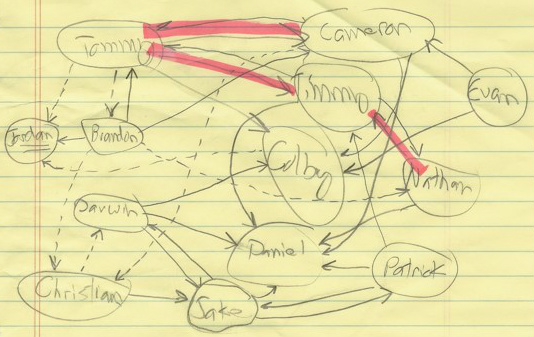
\includegraphics[scale=0.60]{graph}
\end{figure}

The solid arrow represents a preferred companion. For example, there is a solid arrow from Tommy pointing to Colby indicating that Tommy likes to be with Colby. A dashed arrow represents a dislike. For example, there is a dashed arrow from Tommy to Jordan showing that Tommy does not want to be with Jordan. Furthermore, the Scoutmaster provided us a separate email, and indicated that Colby and Jordan cannot be in the same troop. The highlighted arrows in the figure above does not mean anything new between the relationships of the boy scouts.

The Stirling number of the second kind provides the total possible ways to arrange any number of distinguishable objects to indistinguishable groups as long as any troop size is permitted and no possible empty troops. For the data in this project, the Stirling number of the second kind for 13 scouts into 2 troops is 4095. This number provides an upper bound on the possible arrangements for the specific problem tackled in this project.

\section*{Previous Work}
(Currently reading more on Max Flow-Min cut, K-means clustering, Graph clustering: http://www.sciencedirect.com/science/article/pii/S1574013707000020. We will talk about generating random solutions)

\section*{Simplifications}
Ultimately, our goal is to find groups for the scouts that will allow them to grow and be happy in the troop. If we really wanted to fully understand how a group can foster growth in an individual, we would want to consider the astronomical number of aspects about the personalities of each member and how those influence each of the other members given those other members’ astronomically complex personalities. Sociological and psychological literature would need to be studied extensively to learn about these aspects, and experts in the field would most likely be required to collect relevant data for each child, taking several weeks to conduct interviews. At the of the day, given our limited knowledge in this area, we settled with considering a subset of the sociological data between the scouts. We asked each scout which other scouts they liked and which ones they disliked. Now, this is obviously a giant simplification, but the difficulty of gathering more complex information and compiling said information would be too great for the expertise level of anyone involved in solving this problem. Also, this process of gathering data would have to be repeated each year for each new batch of new scouts, and would therefore be a burden on the Scoutmaster to collect a lot of data.

Another simplification is to assume that the quality of a group can be determined by the quality of the relationships between the unique pairs of the group - in other words, the whole is equal to the sum of the parts. For example, consider the case where scouts A, B and C individually like each other when they are alone with one other scout, but don’t like being in a group together. This epiphenomenon won’t be considered; in context of our model, the pairing of these scouts would be heavily favored. 

\section*{Mathematical Model}
To model the relationships between scouts, we use a mathematical graph. We let the scouts be vertices in our graph. A directed edge between Scout A and Scout B has a weight proportional to how much Scout A likes Scout B. We would then like to find a partition of the vertices in the graph that minimizes an objective function given constraints on the sizes of subsets generated by our partition. This results in a complete graph on 13 vertices having edge weights 0, 1, or -1, corresponding to indifference, approval, or disapproval, respectively. Scoutmaster Bruce specifically would like two patrols from the 13 scouts - one of size 6, the other of size 7. The total number of partitions given these constrants is $\binom{13}{6} = \binom{13}{7} = 1716$. This number is reasonable enough that we may calculate the total loss of every valid grouping and select the partition with the lowest score.

We measure the goodness (or score) of a partition in six different ways, corresponding to six different objective functions, which we dub MinCut, FriendCut, EnemyCut, AwkwardCut, and HybridCut. MinCut is designed to minimize the cut edge weights between partitions (see \textit{Solution of Mathematical Problem}). FriendCut is designed to maximize the number of intra-patrol positive edge weights. EnemyCut is meant to minimize the number of intra-patrol negative edge weights, Awkward cut ($+i$) is the same as MinCut, but with an additional penalty of $i$ if there are a pair of scouts, Scout A and Scout B, such that Scout A favors Scout B, but Scout B disfavors Scout A. Hybrid Cut is a convex combination of MinCut and FriendCut, each with equal weight (that is, half the MinCut loss plus half the FriendCut loss). Our three primary objective functions - MinCut, FriendCut, and EnemyCut are given a more rigorous treatment in the next section.

\section*{Solution of Mathematical Problem}
We represent our directed graph as a 13 by 13 similarity matrix, or, as might
be more fitting for the problem, an ``affinity'' matrix. Like below\footnote{The scouts were enumerated like so: 1. Brandon, 2. Cameron, 3, Christian, 4. Colby, 5. Daniel, 6. Darwin, 7. Evan, 8. Jake, 9. Jordan, 10. Nathan, 11. Patrick, 12. Timmy, 13. Tommy.}:

\begin{figure}[h]
    \centering
    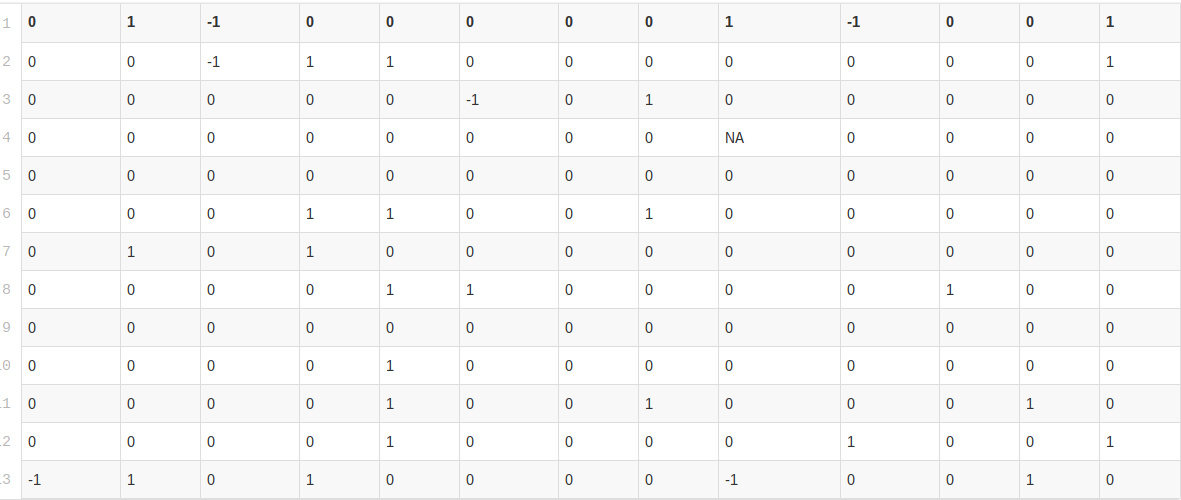
\includegraphics[scale=0.28]{data}
\end{figure}
%%%%%%%%%%%%%%%%%%%%%%%%%%%%%%%%%%%%%%%%%%%%%%%%%%%%%%%%%%%%%%%%%%%%%%%%
%%%%%%%%%%%%%%%%%%%%%%%%%%%%%%%%%%%%%%%%%%%%%%%%%%%%%%%%%%%%%%%%%%%%%%%%

The NA value represents a hard constraint established by a scout's parent (i.e., under no circumstances are these two to be in the same patrol). We designed a number of objective functions that accept two scouts and calculates the loss associated with such a placement. The loss is defined to be $L(x, y) = \text{max}(-2, x[y] + y[x])$ where $x[y]$ is $x$'s disposition towards $y$ and vise versa. For example, if $x$ dislikes $y$ and $y$ dislikes $x$, the loss is -2. If $x$ likes $y$ but $y$ dislikes $x$ the loss is 0. If $x$ and $y$ both like each other, the loss is 2. In mixed cases where the first scout is indifferent to another, but the other likes or dislikes the first scout, the loss is +1 or -1 respectively. We are trying to minimize the loss, so in applying our loss function over the entire dataset, our algorithm is equally averse to same-patrol mutual enmity as it is to dividing mutual friendship, half as averse to the indifference of one scout and the stronger inclination of another, and indifferent to polar opposite affinities within the same patrol. There is a question as to whether this is an accurate reflection of how individual scouts would view their own ``loss'' of any of the possible scenarios. As it turns out, our algorithm arrives at a very reasonable solution regardless. 
\section*{Results}
As mentioned earlier, the number of scouts we must partition is small enough to find an optimal solution by brute force. Our algorithm finds a partition of scouts into patrols of sizes 6 and 7 which is optimal with respect to each objective.

\clearpage

\begin{figure}[h]
\centering
\begin{tabular}{ |l|l|l|l|l|l| }
\hline
\multicolumn{2}{|c|}{\textbf{MinCut}} & \multicolumn{2}{|c|}{\textbf{FriendCut}} & \multicolumn{2}{|c|}{\textbf{EnemyCut}}\\
\hline
Patrol 1 & Patrol 2 & Patrol 1 & Patrol 2 & Patrol 1 & Patrol 2\\
\hline
Brandon & Christian & Brandon & Daniel & Brandon & Christian\\
Cameron & Daniel & Cameron & Darwin & Cameron & Jake\\
Colby & Jake & Christian & Jake & Colby & Jordan\\
Darwin & Jordan & Colby & Jordan  & Daniel & Nathan\\
Evan & Nathan & Evan & Nathan & Darwin & Patrick\\
Tommy & Patrick & Tommy & Patrick & Evan & Timmy\\
& Timmy & & Timmy & Tommy & \\
\hline
\multicolumn{6}{|c|}{\hphantom{1}} \\
\hline
\multicolumn{2}{|c|}{\textbf{AwkwardCut (+1)}} & \multicolumn{2}{|c|}{\textbf{AwkwardCut (+2)}} & \multicolumn{2}{|c|}{\textbf{HybridCut}} \\
\hline
Patrol 1 & Patrol 2 & Patrol 1 & Patrol 2 & Patrol 1 & Patrol 2\\
\hline
Brandon & Christian & Brandon & Cameron & Brandon & Christian\\
Cameron & Daniel & Christian & Evan & Cameron & Daniel\\
Colby & Jake & Daniel & Evan & Colby & Darwin\\
Darwin & Jordan & Darwin & Nathan & Evan & Jake\\
Evan & Nathan & Jake & Timmy & Timmy & Jordan\\
Tommy & Patrick & Jordan & Tommy & Tommy & Nathan\\
\hphantom{1} & Timmy & Patrick & \hphantom{1} & \hphantom{1} & Patrick\\
\hline
\end{tabular}
\caption{The partitions arrived at by minimizing each objective function}
\end{figure}

For each method we define three scoring metrics:

\begin{enumerate}
\item \textbf{MinCut}. This is the traditional metric of a cut on a weighted graph and is the sum of the weights of the edges we would ``cut'' if we were to sever the edges between distinct patrols. More formally, for some partition $I, J$ $I \neq J$, the MinCut is defined as:
$$
MinCut(I, J) := \sum_{e = (i, j), i \in I, j \in J}^{} c(e)
$$
We want this to be as low as possible.
\item \textbf{FriendCut}. This is the sum of the positive, or friendly edge weights within each patrol. That is, if $I_+ = \{e=(i,j) | i,j \in I, c(e)=1\}$ is the the set of edges in patrol $I$ with positive weight and $J_+ = \{e=(i,j) | i,j \in J, c(e)=1\}$ is the set of edges in patrol $J$ with positive weight, then (assuming all positive weights are 1):
$$
FriendCut(I, J) :=  |I_+ \cup J_+|
$$
We want this to be as high as possible.
\item \textbf{EnemyCut}. This is similar to FriendCut, except we now measure the number of negative edges going from one scout to another within the same patrol. Let $I_- = \{e=(i,j) | i,j \in I, c(e)=-1\}$ be the the set of edges in patrol $I$ with negative weight and $J_- = \{e=(i,j) | i,j \in J, c(e)=-1\}$ be the set of edges in patrol $J$ with negative weight, then
$$
EnemyCut(I, J) := |I_- \cup J_-|
$$
    We want this to be as low as possible.
\end{enumerate}

The other methods are modifications of these three and are defined in Appendix A.

\clearpage 

\begin{figure}[h]
    \centering
    \begin{tabular}{ |l|l|l|l| }
        \hline
        \textbf{Method} & \textbf{MinCut} & \textbf{FriendCut} & \textbf{EnemyCut} \\
        \hline
        MinCut & 0 & 17 & 0 \\
        FriendCut & 1 & 18 & 1 \\
        EnemyCut & 2 & 15 & 0 \\
        AwkwardCut (+1) & 0 & 17 & 0 \\
        AwkwardCut (+2) & 1 & 18 & 2 \\
        HybridCut & 0 & 18 & 1 \\
        \hline
    \end{tabular}
    \caption{The scores according to the three primary metrics.}
\end{figure}

Of the objective functions we chose to use, it seems like MinCut and HybridCut are the best performing. FriendCut performs almost as well as HybridCut, except for one worse in the EnemyCut objective. EnemyCut does poorly since finding a partition with 0 intra-patrol negative weight edges is easy in this example, and so EnemyCut settles for the first suboptimal (in terms of the other objective functions) solution it finds. AwkwardCut (+1) arrived at the same partition as MinCut (not altogether surprising, but informative, since even with the additional +1 penalty for placing Brandon and Tommy in the same patrol it decided it would be best off to do so anyways). But changing the ``awkward'' penalty to +2, the same penalty as mutual dislike in EnemyCut, we get a completely different partition.

Let's take a more critical look at the optimal partition arrived at via MinCut:

\begin{table}[h]
	\caption{}\label{eqtable}
	\renewcommand\arraystretch{1.5}
	\noindent\[
	\begin{array}{|c|c|}
	\hline
	\textbf{Patrol 1}&\textbf{Patrol 2}\\
	\hline
	\text{Brandon, Cameron, Colby,}&\text{Christian, Daniel, Jake,}\\
	\text{Darwin, Evan, Tommy}&\text{Jordan, Nathan, Patrick, Timmy}\\
	\hline
	\end{array}
	\]
\end{table}

\begin{enumerate}
	\item Tommy and Timmy both like each other and are in separate patrols. But if we move Timmy to Patrol 1 ($P1$), we break up the mutual friendship of Timmy and Nathan in $P2$. Suppose we moved both Timmy and Nathan to $P1$ and Brandon (who dislikes Nathan) to $P2$. But then Brandon loses two friends (Tommy and Cameron), gains one (Jordan), and now neither Nathan nor Timmy are in the same patrol as Daniel, whom they both like. Although, Brandon and Tommy find themselves in the awkward situation of having complete opposite sentiments towards each other. Perhaps this would be a worthwhile trade after all (and a larger, negative weight needs to be placed upon disfavor-favor relationships).
	
	\item As mentioned in the previous point, Tommy dislikes Brandon. Trading Tommy in $P1$ for Jordan in $P2$ seems promising, But we have overlooked the fact that Colby and Jordan are our NA pair, and cannot be in the same patrol under any circumstances. Trading Colby for Jordan is another option, but Colby will be missed by Darwin, Evan, Cameron and Tommy (In other words, the whole of P1 minus Brandon).
\end{enumerate}

On the whole, though, there are no obvious improvements that can be made to our algorithm's partition. We find that this is an assignment that could have reasonably been arrived at by Scoutmaster Bruce (granted the group dynamics have not changed since the scouts were surveyed).  Furthermore, the solution took only 10 seconds to arrive at on a single core machine.

\section*{Improvements}
While our algorithm demonstrably works well on smaller groups of 13 people, we do not expect our brute force solution to be tractable on larger groups wherein greater than 2 partitions are required. As a possible scenario, consider a company of 150 people to be divided into fixed-size teams of 10 individuals each. There are $150! / (10!)^{15}$ possible partitions, a number proportional to $10^{164}$ - meaning we could instead use that computational time to enumerate the number of atoms in the universe… a tredecillion $(10^{78})$ times. Knowing this, perhaps it won’t surprise the reader that this particular graph partitioning problem in general graphs is NP-complete - though there do exist approximation algorithms.%
%%%%%%%%%%%%%%%%%%%%%%%%%%%%%%%%%%%%%%%%%%%%%%%%%%%%%%%%%%%%%%%%%%%%%%%%
\footnote{B. W. Kernighan, S. Lin, \textit{An Efficient Heuristic Procedure for Partitioning Graphs}. Bell System Technical Journal. \textbf{49} (1970), 291--307. doi: 10.1002/j.1538-7305.1970.tb01770.x}%
%%%%%%%%%%%%%%%%%%%%%%%%%%%%%%%%%%%%%%%%%%%%%%%%%%%%%%%%%%%%%%%%%%%%%%%%
As scout enrollment increases, it becomes necessary to consider scenarios where we have both a large number of scouts in need of assignment and multiple patrols to choose from. Our algorithm could be extended to use brute force to find a globally optimal solution when it is deemed computationally feasible and to use an approximating algorithm to find a locally optimal solution otherwise. 

\section*{Conclusions}
We initially struggled to decide on determining an appropriate objective function to partition the scouts to different groups. Follow up interviews with Scoutmaster Gene Bruce allowed us to decide on this function. We learned to rely on his expertise and intuition rather than trying to blindly decide on which types of relationships should be fostered and avoided to weight our objective function. Thus, we learned necessary communication skills and consideration of our community partner's needs.

With a feasibility check of how many solutions possible once the mathematical model was decided using graphs, a brute force strategy was the most accessible method to arrive at a solution. Thus we were able to develop a program that can partition scouts using this strategy. We learned to utilize tools we have at hand right away, and then we can consider other methods later on to reduce the computational time of our algorithm.

\section*{Acknowledgments}
We would like to thank Scoutmaster Gene Bruce for providing us the necessary data and being extremely patient and understanding when discussing the background and problem. We would also like to thank Professor Sarah Billey for the mentorship and guidance she provided throughout this project, and our TA Austin Tran for his comments and suggestions. 

\section*{Verification Statement}
(Once we receive our verification statement, we will place it here.)

\section*{Appendix A}
The other objective functions.

\begin{enumerate}
    \item \textbf{AwkwardCut (+i)}. Same in all respects to MinCut, except for an additional penalty of $i$ if there are two scouts, Scout A and Scout B, in the same patrol such that Scout A likes Scout B and Scout B dislikes Scout A.
    \begin{equation*}
        \begin{split}
            AwkwardCut&(I, J, i) := \Bigg[ \sum_{e = (k, j), k \in I, j \in J}^{} c(e) \Bigg] \\
            &+ i * \left\vert{\{e_+ = (k,j), e_- = (j, k) : e_+, e_- \in I, c(e_+) = 1, c(e_-) = -1\}}\right\vert
        \end{split}
    \end{equation*}

\item \textbf{HybridCut}. A convex combination of MinCut and FriendCut, each with equal weight (that is, half the MinCut loss plus half the FriendCut loss).
    \begin{equation*}
        HybridCut(I, J) := \frac{1}{2}MinCut(I, J) + \frac{1}{2}FriendCut(I, J)
    \end{equation*}
\end{enumerate}

\section*{Appendix B}
The solution for finding the Stirling number of the second kind for $n = 13$ scouts to be arranged in $k = 2$ troops:
\begin{gather*}
	S(n,k) = \frac{1}{k!} \sum_{i=0}^{k}(-1)^k {2 \choose i} (k - i)^{n} \\
	S(13,2) = \frac{1}{2!} \sum_{i=0}^{2}(-1)^2 {2 \choose i} (2 - i)^{13} \\
	S(13, 2) = 4095
\end{gather*}

\bibliographystyle{amsplain}
\begin{thebibliography}{10}

\bibitem {A} B. W. Kernighan, S. Lin, \textit{An Efficient Heuristic Procedure for Partitioning Graphs}. Bell System Technical Journal. \textbf{49} (1970), 291--307. doi: 10.1002/j.1538-7305.1970.tb01770.x

\end{thebibliography}

\end{document}

%------------------------------------------------------------------------------
% End of journal.tex
%------------------------------------------------------------------------------
=======

\documentclass{amsart}

%     If your article includes graphics, uncomment this command.
\usepackage{graphicx}
\usepackage{amsmath,amsfonts,amssymb,amscd,amsthm,amsbsy,upref}
\usepackage[all]{xy}
\usepackage{amsmath}
\usepackage{mathrsfs}
\usepackage{paralist}
\usepackage{setspace}
\usepackage{graphicx}
\usepackage{tikz-cd}
\usepackage{pgfplots}
\usepackage{fancyhdr}
\usepackage{tikz}
\usepackage{pgfplots}
\usepackage{array}

\newtheorem{theorem}{Theorem}[section]
\newtheorem{lemma}[theorem]{Lemma}

\theoremstyle{definition}
\newtheorem{definition}[theorem]{Definition}
\newtheorem{example}[theorem]{Example}
\newtheorem{xca}[theorem]{Exercise}

\theoremstyle{remark}
\newtheorem{remark}[theorem]{Remark}

\numberwithin{equation}{section}

%    Absolute value notation
\newcommand{\abs}[1]{\lvert#1\rvert}

%    Blank box placeholder for figures (to avoid requiring any
%    particular graphics capabilities for printing this document).
\newcommand{\blankbox}[2]{%
  \parbox{\columnwidth}{\centering
%    Set fboxsep to 0 so that the actual size of the box will match the
%    given measurements more closely.
    \setlength{\fboxsep}{0pt}%
    \fbox{\raisebox{0pt}[#2]{\hspace{#1}}}%
  }%
}

\pgfplotsset{compat=1.13}

\begin{document}

\title{Assigning Scouts to Optimal Patrols}
\author{Phil Snyder}
\author{Ian Bruce}
\author{Julio Marco Pineda}

\begin{abstract}
The Scoutmaster wants to find an arrangement of 13 new scouts into two patrols. The cohesiveness and overall quality experience of a patrol is severely affected by adverse relationship and can be improved by existing preferences. Thus, by using anonymous data from scouts and parents, a brute force strategy was employed to find the optimal arrangement of scouts that avoids severe conflict and maximizes existing preferences. An arrangement of 6 and 7 scouts on one patrol respectively was found that satisfies the desired conditions. 
\end{abstract}
\maketitle
\section*{Problem Description}
Every year the Scoutmaster must assign new scouts to groups called patrols. In these patrols, scouts would plan and perform different scouting activities together in which they can form close friends that grow together. However, in recent years, the number of scouts have been increasing at a rate such that it is no longer logistically viable to place every new scout in a single patrol; multiple patrols are needed to organize activities better and to form proper bonds and community between the new recruits. Furthermore, the new scouts are in the fifth or sixth grade who have not fully developed their interpersonal skills. Many can be temperamental and awkward when dealing with adversity, and even some devastating conflicts occur where not only the two fighting scouts create animosity between each other, the rest of the troop alienates the destructive pair. If enough of these adverse interactions occur within a troop, many scouts would decide to quit and lose out in a great experience and community in the Boy Scouts.

The data the scoutmaster collects about adverse pairings and preferences are either privately given by the scouts themselves or by their parents. The possibly destructive interactions are given by the parents of the scouts.Previously, the Scoutmaster was able to determine the perfect patrols manually due to having smaller number of scouts. However, the number of scouts have been increasing yearly to the point that solving this grouping problem cannot be done by hand in a reasonable time. Therefore, we can help our community partner find a better means to solve his troop organization problem. Our goal for this project is to assign boy scouts in different patrols of appropriate size (of 6-8 scouts) such that we maximize the retention rate of the scouts in the program by avoiding severe conflicts while maximizing positive relationships between scouts.

We would like to answer the direct problem our community partner provided of arranging 15 scouts into two troops that avoids severe conflicts and promotes the positive relationships between the scouts. Furthermore, we want to determine if we can build a model to predict these patrol arrangements for any number of scouts so that the Scoutmaster can use this model for future years. Other than improving the overall experience of the scouts and alleviating the burden of the Scoutmaster, this model can possibly be applied to other situations where arranging a number of people of groups where interpersonal dynamics is necessary and important.

\section*{Simplifications}
Ultimately, our goal is to find groups for the scouts that will allow them to grow and be happy in the troop. If we really wanted to fully understand how a group can foster growth in an individual, we would want to consider the astronomical number of aspects about the personalities of each member and how those influence each of the other members given those other members’ astronomically complex personalities. Sociological and psychological literature would need to be studied extensively to learn about these aspects, and experts in the field would most likely be required to collect relevant data for each child, taking several weeks to conduct interviews. At the of the day, given our limited knowledge in this area, we settled with considering a subset of the sociological data between the scouts. We asked each scout which other scouts they liked and which ones they disliked. Now, this is obviously a giant simplification, but the difficulty of gathering more complex information and compiling said information would be too great for the expertise level of anyone involved in solving this problem. Also, this process of gathering data would have to be repeated each year for each new batch of new scouts, and would therefore be a burden on the Scoutmaster to collect a lot of data.

Another simplification is to assume that the quality of a group can be determined by the quality of the relationships between the unique pairs of the group - in other words, the whole is equal to the sum of the parts. For example, consider the case where scouts A, B and C individually like each other when they are alone with one other scout, but don’t like being in a group together. This epiphenomenon won’t be considered; in context of our model, the pairing of these scouts would be heavily favored. 

\section*{Mathematical Model}
This problem visually lends itself well to the notion of a mathematical graph. Since there is an inherent sense of relationships between individuals (how much a scout likes another scout), it is appropriate to consider the scouts as vertices in a graph with directed edges representing how much the “head” scout likes the “tail” scout. Our goal, using this language, is to find a partition of the vertices in the graph that satisfies some sort of objective function given size constraints of the partitions. In our problem at hand, we consider a complete graph with 13 vertices and edge weights being either 0, 1, or -1, corresponding to indifference, approval, or disapproval respectively of the “head” scout with respect to the “tail” scout. The Scoutmaster specifically wants two groups out of these 13, and with the size constraints for a patrol considered, our goal becomes finding 6 vertices to be in one partition and the other 7 being in another. The total number of partitions becomes 13 choose 6, which is equivalent to 1,716. This is certainly within the scope of considering total enumeration of the partitions as a reasonable solution to the problem, therefore we will proceed accordingly and implement the calculation using Python and its associated libraries to represent the data in a format that is convenient to work with.

Now, a natural question for us to consider is what objective function would be most appropriate to optimize. A natural answer to this would be to sum the edge weights of all edges that connect vertices that are within partitions. This would make sense if separating enemies is just as important as joining friends, but this just might not be the case. In terms of weighing these factors, we defer to Scoutmaster Bruce’s experience with how past patrols fared with friends and foes in the mix. Therefore, we consider a family of possible objective functions, namely giving real numbered weights to instances of approving relationships and disapproving relationships, and select a few of these objective functions to solve for. We then present the collection of results from different objective functions to the Scoutmaster for him to see which one seems to most reasonably match his preferences.
\section*{Solution of Mathematical Problem}
We represent our directed graph as a 13 by 13 similarity matrix, or, as might be more fitting for the problem, an “affinity” matrix. Like below:%
%%%%%%%%%%%%%%%%%%%%%%%%%%%%%%%%%%%%%%%%%%%%%%%%%%%%%%%%%%%%%%%%%%%%%%%%
\footnote{The scouts were enumerated like so: 1. Brandon, 2. Cameron, 3, Christian, 4. Colby, 5. Daniel, 6. Darwin, 7. Evan, 8. Jake, 9. Jordan, 10. Nathan, 11. Patrick, 12. Timmy, 13. Tommy.}%
%%%%%%%%%%%%%%%%%%%%%%%%%%%%%%%%%%%%%%%%%%%%%%%%%%%%%%%%%%%%%%%%%%%%%%%%
\includegraphics[scale=0.6]{solution1.JPG}

The NA value represents a hard constraint established by a scout’s parent (i.e., under no circumstances are these two to be in the same patrol). In our implementation we convert the NA value to $-\infty$. We designed an objective function that accepts two scouts who are assumed to be in different patrols and calculates the loss associated with such a placement. The loss is defined to be $L(x, y) = \text{max}(-2, x[y] + y[x])$ where $x[y]$ is $x$’s disposition towards $y$ and vise versa. For example, if $x$ dislikes $y$ and $y$ dislikes $x$, the loss is -2. If $x$ likes $y$ but $y$ dislikes $x$ the loss is 0. If $x$ and $y$ both like each other, the loss is 2. In mixed cases where the first scout is indifferent to another, but the other likes or dislikes the first scout, the loss is +1 or -1 respectively. We are trying to minimize the loss, so in applying our loss function over the entire dataset, our algorithm is equally averse to same-patrol mutual enmity as it is to dividing mutual friendship, half as averse to the indifference of one scout and the stronger inclination of another, and indifferent to polar opposite affinities within the same patrol. There is a question as to whether this is an accurate reflection of how individual scouts would view their own “loss” of any of the possible scenarios. As it turns out, our algorithm arrives at a very reasonable solution regardless. 
\section*{Results}
As mentioned earlier, the number of scouts we must partition is small enough to find an optimal solution by brute force. Our algorithm finds a partition of scouts into patrols of sizes 6 and 7 with a total loss of 0 as described in the table below:
\begin{table}[ht]
	\caption{}\label{eqtable}
	\renewcommand\arraystretch{1.5}
	\noindent\[
	\begin{array}{|c|c|}
	\hline
	\textbf{Patrol 1}&\textbf{Patrol 2}\\
	\hline
	\text{Brandon, Cameron, Colby,}&\text{Christian, Daniel, Jake,}\\
	\text{Darwin, Evan, Tommy}&\text{Jordan, Nathan, Patrick, Timmy}\\
	\hline
	\end{array}
	\]
\end{table}
\includegraphics[scale=0.65]{results1.JPG}
Of the undesirable outcomes of such a partition, we can spot a few:
\begin{enumerate}
	\item Tommy and Timmy both like each other and are in separate patrols. But if we move Timmy to Patrol 1 ($P1$), we break up the mutual friendship of Timmy and Nathan in $P2$. Suppose we moved both Timmy and Nathan to $P1$ and Brandon (who dislikes Nathan) to $P2$. But then Brandon loses two friends (Tommy and Cameron), gains one (Jordan), and now neither Nathan nor Timmy are in the same patrol as Daniel, whom they both like. Although, Brandon and Tommy find themselves in the awkward situation of having complete opposite sentiments towards each other. Perhaps this would be a worthwhile trade after all (and a larger, negative weight needs to be placed upon disfavor-favor relationships).
	
	\item As mentioned in the previous point, Tommy dislikes Brandon. Trading Tommy in $P1$ for Jordan in $P2$ seems promising, But we have overlooked the fact that Colby and Jordan are our NA pair, and cannot be in the same patrol under any circumstances. Trading Colby for Jordan is another option, but Colby will be missed by Darwin, Evan, Cameron and Tommy (In other words, the whole of P1 minus Brandon).
\end{enumerate}
On the whole, though, there are no obvious improvements that can be made to our algorithm’s partition. We find that this is an assignment that could have reasonably been arrived at by Scoutmaster Bruce (granted the group dynamics have not changed since the scouts were surveyed).  Furthermore, the solution took only 20 seconds to arrive at on a single core machine.

\section*{Improvements}
While our algorithm demonstrably works well on smaller groups of 13 people, we do not expect our brute force solution to be tractable on larger groups wherein greater than 2 partitions are required. As a possible scenario, consider a company of 150 people to be divided into fixed-size teams of 10 individuals each. There are $150! / (10!)^{15}$ possible partitions, a number proportional to $10^164$ - meaning we could instead use that computational time to enumerate the number of atoms in the universe… a tredecillion $(10^{78})$ times. Knowing this, perhaps it won’t surprise the reader that this particular graph partitioning problem in general graphs is NP-complete - though there do exist approximation algorithms.%
%%%%%%%%%%%%%%%%%%%%%%%%%%%%%%%%%%%%%%%%%%%%%%%%%%%%%%%%%%%%%%%%%%%%%%%%
\footnote{B. W. Kernighan, S. Lin, \textit{An Efficient Heuristic Procedure for Partitioning Graphs}. Bell System Technical Journal. \textbf{49} (1970), 291--307. doi: 10.1002/j.1538-7305.1970.tb01770.x}%
%%%%%%%%%%%%%%%%%%%%%%%%%%%%%%%%%%%%%%%%%%%%%%%%%%%%%%%%%%%%%%%%%%%%%%%%
As scout enrollment increases, it becomes necessary to consider scenarios where we have both a large number of scouts in need of assignment and multiple patrols to choose from. Our algorithm could be extended to use brute force to find a globally optimal solution when it is deemed computationally feasible and to use an approximating algorithm to find a locally optimal solution otherwise. 

\section*{Conclusions}
We initially struggled deciding on an appropriate objective function to partition the scouts to different groups. Follow up interviews with Scoutmaster Gene Bruce allowed us to decide on this function. We relied on his expertise and intuition rather than trying to blindly decide on which types of relationships should be fostered and avoided to determine our objective function. Thus, we learned necessary communication skills and consideration of our community partner's needs.

With a feasibility check of how many solutions possible once the mathematical model was decided using graphs, a brute force strategy was the most reliable method to arrive at a solution. Thus we were able to develop a program that can partition scouts using this strategy. We learned to utilize tools we have at hand. Further consideration of other methods later on to reduce the computational time of our algorithm.

\section*{Acknowledgments}
We would like to thank Scoutmaster Gene Bruce for providing us the necessary data and being extremely patient and understanding when discussing the background and problem. We would also like to thank Professor Sara Billey for the mentorship and guidance she provided throughout this project, and our TA Austin Tran for his comments and suggestions. 

\section*{Verification Statement}
(Once we receive our verification statement, we will place it here.)



\bibliographystyle{amsplain}
\begin{thebibliography}{10}

\bibitem {A} B. W. Kernighan, S. Lin, \textit{An Efficient Heuristic Procedure for Partitioning Graphs}. Bell System Technical Journal. \textbf{49} (1970), 291--307. doi: 10.1002/j.1538-7305.1970.tb01770.x

\end{thebibliography}

\end{document}

%------------------------------------------------------------------------------
% End of journal.tex
%------------------------------------------------------------------------------
